\section{Principle Component Analysis (PCA)}
There are many different approaches to identify music by extracting different audio features as
discussed in the Chapter \ref{chapter:lit_review}. Since there are very low number of researches
conducted on sinhala music identification, finding audio features which can differentiate two 
sinhala songs was required to continue the research. Hence \ac{pca} was conducted to find features
on a 5000 song dataset extracting 27 different audio features and results were collected for 
different normalization techniques. \ac{svd} is used to composite multi-dimension features.

\subsection{PCA with Raw Dataset}

Initially a \ac{pca} executed on the raw feature matrix without any normalization technique
which led to the results in Figure \ref{fig:pca_coeff}. Abnormality of the result caused to 
revisit the feature matrix and need of a normalization technique was identified. 

\begin{figure}[H]
    \centering
    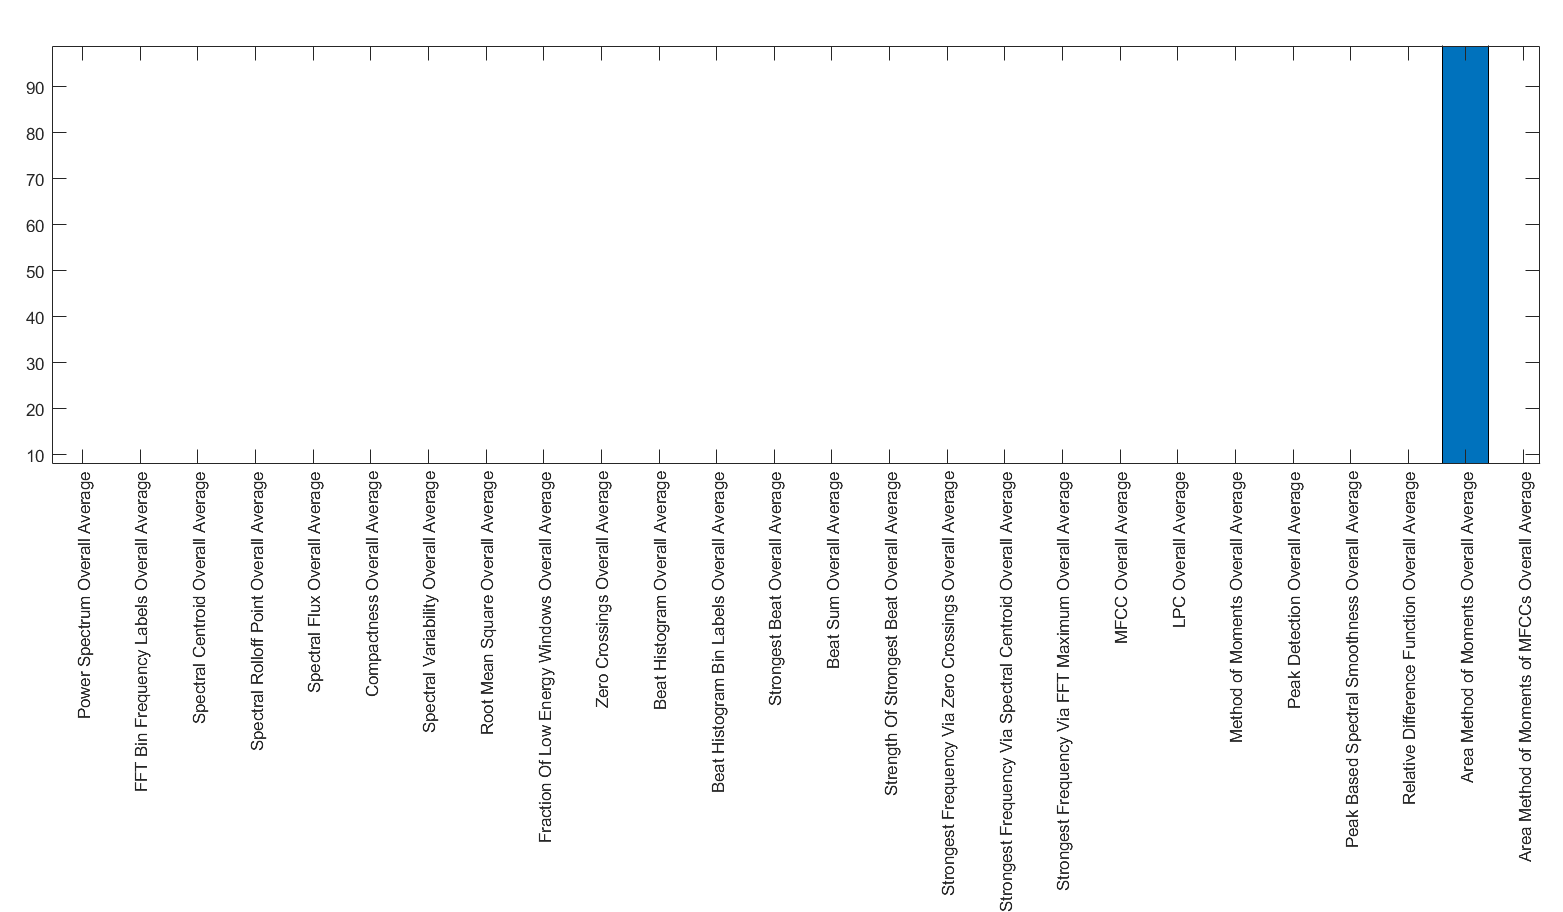
\includegraphics[scale=0.35]{pca_coeff.png}
    \caption{PCA coefficients weighted by eigen values}
    \label{fig:pca_coeff}
\end{figure}

\subsection{PCA with Dataset Normalized by Z-score}

Then \ac{pca} conducted on the dataset which was normalized by z-score. Which produced results
on Figure \ref{fig:pca_coeff_z}. While analyzing the results, it was observed that results
indicate uniform variance among the features that was not present in the original feature
matrix. Hence need of a normalization technique which preserve the variance of a feature 
identified. 

\begin{figure}[H]
    \centering
    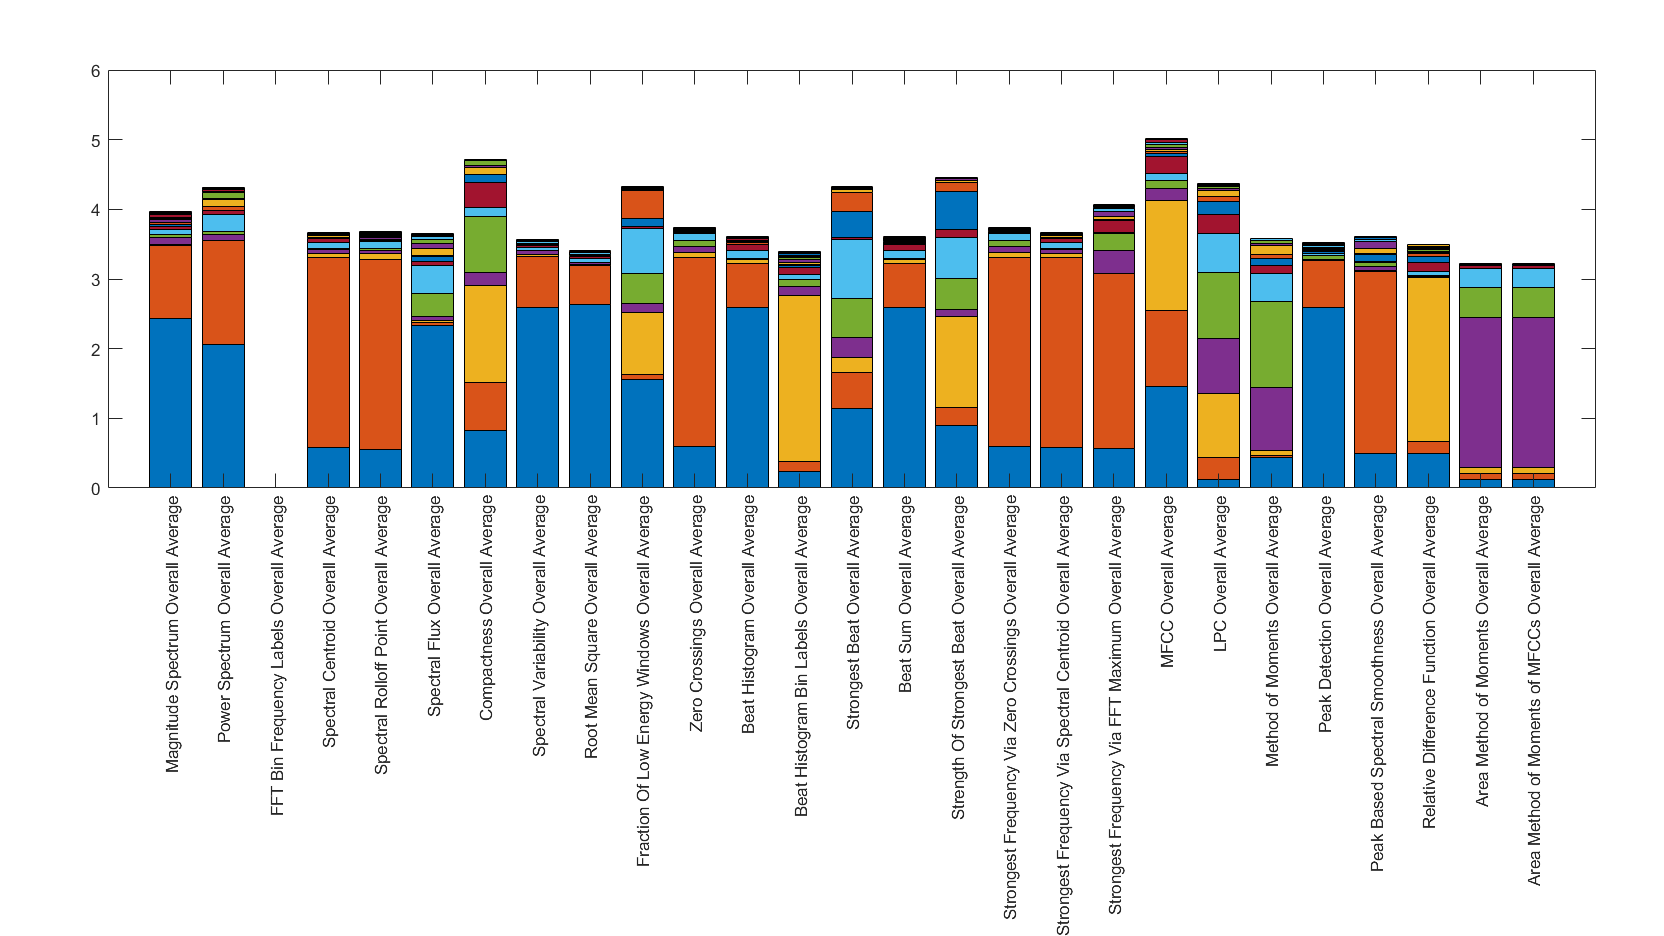
\includegraphics[scale=0.35]{pca_coeff_z.png}
    \caption{PCA coefficients weighted by eigen values (Normalized by Zscore)}
    \label{fig:pca_coeff_z}
\end{figure}

\subsection{PCA with Dataset Normalized by Rescaling}

Finally dataset was normalized by rescaling and conducted \ac{pca} gave a justifiable result
which is shown in the Figure \ref{fig:pca_coeff_z}. \say{Area Method of Moments} and \say{Area 
Method of Moments of MFCCs} have identified as the two features which covers majority of variance
in the dataset. 

\begin{figure}[H]
    \centering
    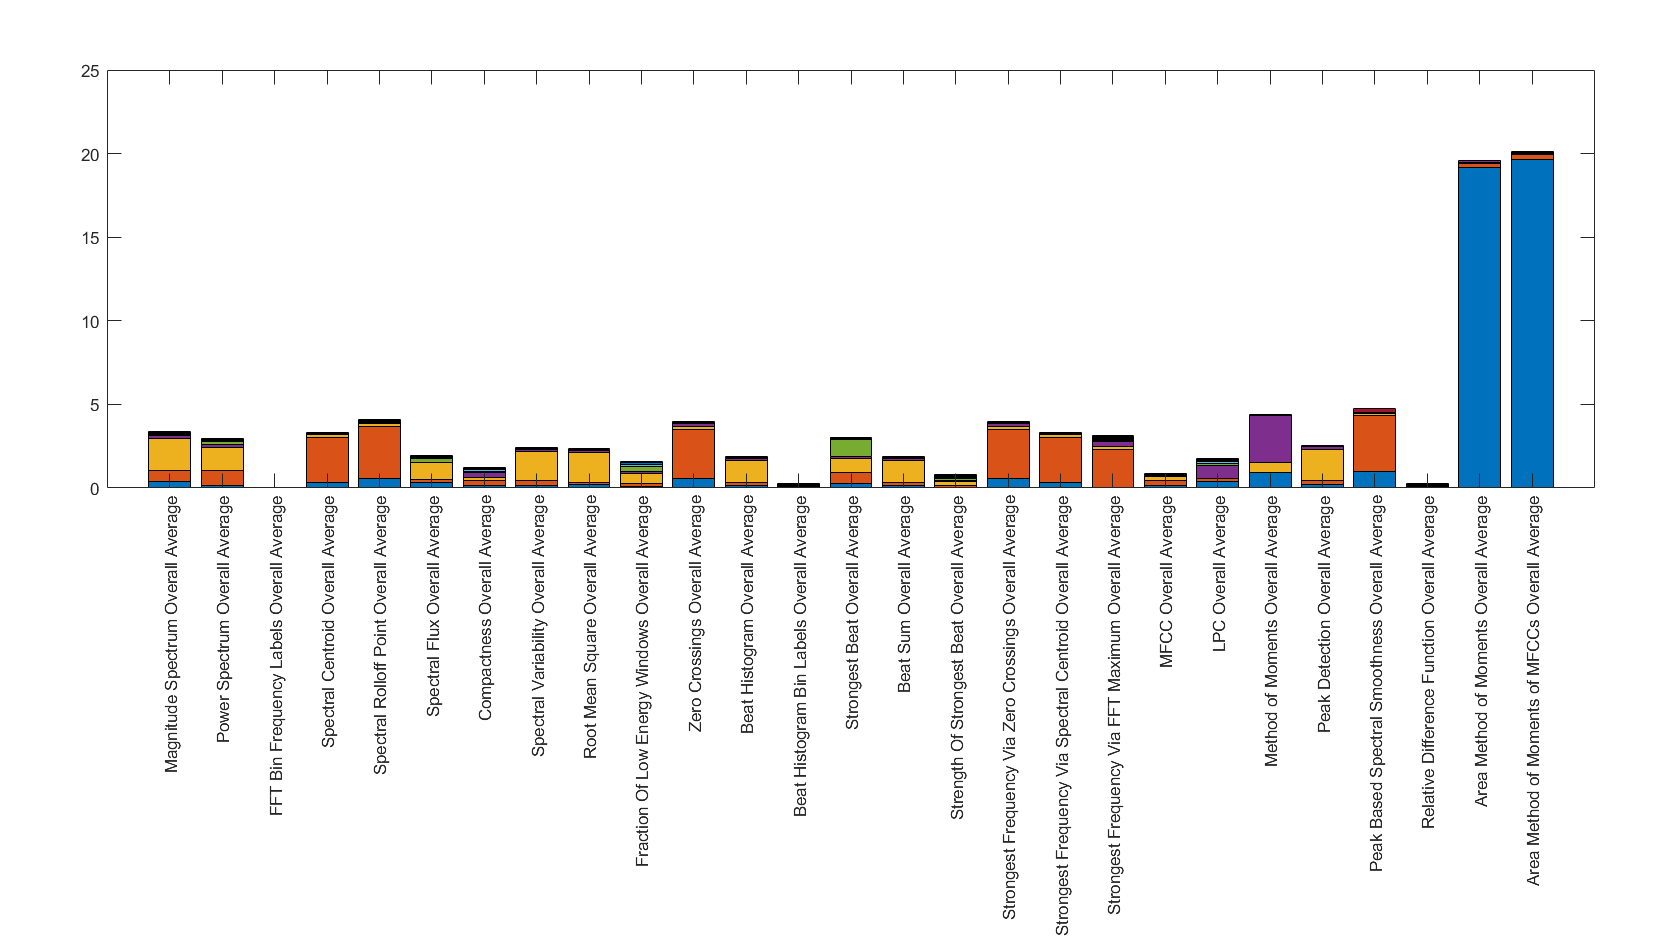
\includegraphics[scale=0.35]{pca_coeff_re.png}
    \caption{PCA coefficients weighted by eigen values (Normalized by Rescaling)}
    \label{fig:pca_coeff_re}
\end{figure}

Then those two features were extracted from audio clips with slight changes to tempo and pitch, in order 
to check whether those two features show any invariance to pitch or tempo. But when tempo or pitch changed
slightly, \ac{svd} values of those features changed drastically. Therefore results of the \ac{pca} couldn't
be used to progress on this research which resulted to revisit the literature to find better features to 
extract. 